\section{Protocolo de Incentivos para Desarrolladores (\textit{Developer Incentive Protocol}, DIP)}
\label{sec:dip}

\subsection{Metas de diseño}
\label{dip:design}

Con el fin de crear una comunidad atractiva en Nebulas proponemos la puesta en servicio del Protocolo de Incentivos para Desarrolladores (DIP) —destinado a programadores de contratos inteligentes en Nebulas— que recompensa con NAS a los más destacados.

\subsection{Algoritmo de distribución de recompensas}
\label{dip:arith}

Creemos que un buen contrato inteligente depende de la cantidad de usuarios que están dispuestos a usarlo. A mayor cantidad de cuentas con buena valuación, mejor será el contrato inteligente. Se utiliza Nebulas Rank a modo de criterio de valuación universal de dichas cuentas. El diseño de DIP combina NR y el concepto común de WAA (\textit{Weekly Active Addresses}, o Direcciones Activas Semanalmente), y el valor WAA total obtenido se utiliza para la valuación del contrato inteligente.

El cómputo del DIP se realiza semanalmente. Para un contrato inteligente \textit{C}, asumimos que el conjunto de direcciones de cuenta activas de esa semana es WAA (\textit{Weekly Active Acounts}). Según la valuación NR en \refsec{subsec:leaderrank} (se toman las diez principales), la suma de los valores NR de las direcciones activas esa semana se calcula como el SCS (\textit{Smart Contracts Score}, o Puntaje de Contratos Inteligentes) del Contrato C, tal como se muestra en la ecuación \ref{formula:dip:scs}.

\begin{align}
\label{formula:dip:scs}
SCS(C)=\sum_{addr \in WAA}(max\{X + 1 - NR(addr), 0\})
\end{align}

Con base en el cómputo semanal de SCS (Puntaje de Contratos Inteligentes), las recompensas se clasifican de mayor a menor de acuerdo a su SCR (\textit{Smart Contract Rank}, Valuación de Contratos Inteligentes). Se toman los mejores $N$ contratos inteligentes, de las cuales sus desarrolladores compartirán $M$ NAS en concepto de recompensas, y en forma proporcional al SCR. Con el fin de evitar manipulaciones en la clasificación, la curva de distribución DIP está diseñada para ser uniforme como se muestra en \reffig{fig:dipdis}, pero aún así se asegura que los ingresos de la valuación 1 sean 2 veces mayores que los de la valuación $N$ para indicar la diferencia en SCS. Las restricciones de proporción se muestran en la ecuación \ref{formula:dip}.

\begin{alignat}{2}
Coin(C) = & \quad kln(N+1-SCR(C))+b \label{formula:dip} \\
\mbox{s.t.}\quad & kln(N) + b = 2b \nonumber \\
& \sum_{x=1}^{N}(kln(x) + b) = M \nonumber
\end{alignat}

\begin{figure}[h]
\centering
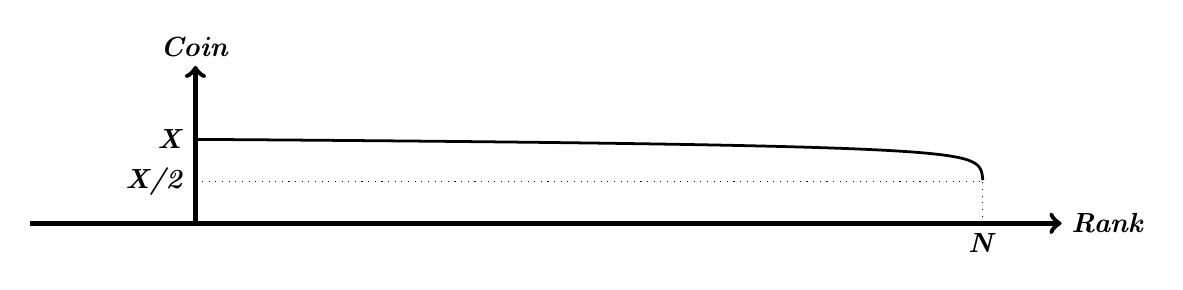
\begin{tikzpicture}
\coordinate (OR) at (0.00, 0.00);
\coordinate (LX) at (-2.10, 0.00); % left x
\coordinate (RX) at (11.00, 0.00); % right x
\coordinate (BY) at (0.00, 0.00); % bottom y
\coordinate (TY) at (0.00, 2.00); % top y
\draw[->][line width=1.75pt] (LX) -- (RX);
\node[right,black] at (11,0) {\textbf{\textit{Rank}}};
\draw[->][line width=1.75pt] (BY) -- (TY);
\node[above,black] at (0, 2) {\textbf{\textit{Coin}}};
\draw[dotted] (0,0.533210267)--(10,0.533210267);
\draw[dotted] (10,0)--(10,0.533210267);
\node[below,black] at (10, 0) {\textbf{\textit{N}}};
\node[left,black] at (0, 0.533210267) {\textbf{\textit{X/2}}};
\node[left,black] at (0, 1.066420536) {\textbf{\textit{X}}};
\draw[black, line width=1.00pt, domain=0:10.00,samples=3000] plot[smooth](\x, {.066598275 * ln(3001-\x * 300) + .533210267});
\end{tikzpicture}
\caption{Curva de distribución de recompensas DIP}
\label{fig:dipdis}
\end{figure}

Las recompensas DIP se calcularán separadamente y serán distribuidas por cada nodo. Asumiendo que un bloque dado se genera cada S segundos (s), las recompensas DIP se calcularán una vez cada 24*7*3600/S bloques para todos los nodos, y serán distribuidas a las direcciones de retiros de los contratos inteligentes.

Con el fin de fomentar la diversidad de los contratos inteligentes de Nebulas y estimular buenos resultados por parte de más desarrolladores, DIP estipula que cada contrato inteligente puede ser recompensado hasta K tiempo(s). DIP seleccionará los mejores $N$ contratos inteligentes cualificados para recibir recompensas de acuerdo a su valuación, con el fin de promover el desarrollo de la construcción de aplicaciones blockchain en el ecosistema.

\subsection{Resultados experimentales}
\label{dip:economic}

Recopilamos los datos de las transacciones realizadas en mayo de 2017 en la red Ethereum y calculamos la clasificación DIP de la primera semana, como se muestra en la tabla \ref{table:dip}.

\begin{table}[h]
\centering
\begin{threeparttable}[b]
\caption{Los mejores 10 resultados de la valuación DIP de la primera semana de mayo de 2017\tnote{1}}
\label{table:dip}
\begin{tabular}{ccc} \toprule
    {Dirección del contrato} & {Puntuación} & {Descripción\tnote{2}} \\ \midrule
0xa74476443119a942de498590fe1f2454d7d4ac0d & 264456363.0 & GolemToken \\
0x49edf201c1e139282643d5e7c6fb0c7219ad1db7 & 207900181.0 & TokenCard-ICO \\
0x48c80f1f4d53d5951e5d5438b54cba84f29f32a5 & 129625776.0 & REP-Augur-OLD \\
0x6810e776880c02933d47db1b9fc05908e5386b96 & 108324489.0 & Gnosis-TokenContract \\
0x6090a6e47849629b7245dfa1ca21d94cd15878ef & 54429341.0 & ENS-Registrar \\
0x607f4c5bb672230e8672085532f7e901544a7375 & 48526808.0 & RLC \\
0x8d12a197cb00d4747a1fe03395095ce2a5cc6819 & 46498412.0 & etherdelta\_2 \\
0xf7b098298f7c69fc14610bf71d5e02c60792894c & 43746158.0 & GUPToken \\
0xaaaf91d9b90df800df4f55c205fd6989c977e73a & 42026627.0 & TokenCardContract \\
0xaec2e87e0a235266d9c5adc9deb4b2e29b54d009 & 41427314.0 & singularDTVToken \\
\bottomrule
\end{tabular}
\begin{tablenotes}
  \small
  \item[1] rango de los bloques: [3629091, 3665815]
  \item[2] datos tomados de etherscan.io
\end{tablenotes}
\end{threeparttable}
\end{table}

Se puede ver que los contratos de mayor rango son más visibles y activos en el ciclo de cálculo, lo que está en línea con nuestra intención original de motivar a los constructores del ecosistema.

\subsection{Análisis de fraudes}
\label{dip:sybil}

Los contratos inteligentes sólo se pueden llamar de forma pasiva. En consecuencia, si un estafador desea incrementar la valuación de su contrato inteligente, tendrá que encontrar cuentas con una valuación NR lo suficientemente altas que realicen llamadas a su contrato.

En primer lugar, será imposible para los estafadores mejorar su clasificación DIP de forma gratuita. Se asume que ellos buscarán mejorar su posición en el Contrato C mediante la creación de un gran número de cuentas para ello. Sin embargo, cuando el SCS se calcula en la ecuación \ref{formula:dip:scs}, sólo los $N$ mejores SCS en el ranking NR obtendrán una valuación mayor a 0, mientras que el ranking NR de las nuevas cuentas estará fuera de esa clasificación. Incluso si realiza llamadas al Contrato C desde las cuentas, no habrá ningún impacto en la valuación DIP.

En segundo lugar, si el estafador está dispuesto a pagar una cierta suma para mejorar la valuación DIP de su contrato, tiene sólo dos alternativas su alcance. La primera de ellas es crear cuentas con una valuación NR alta y realizar llamadas al Contrato C por su cuenta. Este escenario ha sido analizado para la creación de cuentas con alta valuación NR en \refsec{subsec:robust}. Para mejorar la valuación NR en cada una de sus cuentas —mediante la alteración de su topología— necesitará una gran cantidad de dinero. Más allá de eso, debido a que NR se actualiza periódicamente, le resultará muy costoso mantener alta su valuación NR. La segunda alternativa es encontrar un gran número de cuentas cuya valuación NR sea alta, y persuadir o sobornar a sus propietarios para que realicen llamadas al Contrato C. Esta acción, sin embargo, es muy difícil de llevar a cabo a gran escala. Lo que es peor, aquellas cuentas con alto valor NR representarán únicamente un pequeño porcentaje de las mejores $N$, lo que representará, globalmente, un impacto casi nulo en contratos legítimamente sobresalientes.